%!TEX root = ../../ClassicThesis.tex
%-------------------------------------------------------------------------------
\section{Introduction}
%-------------------------------------------------------------------------------

%-------------------------------------------------------------------------------
\section{Results}
%-------------------------------------------------------------------------------

%-------------------------------------------------------------------------------
\FloatBarrier
\subsection{Signal and Noise Correlation}

\marginpar{Take text from supplemental materials for paper, but here with the addition of phase correlating with itself and with power.}

\begin{figure}[htb]
    \centering
    \subfloat[Signal correlation\label{fig:lam_signal_corr_depth}]{
        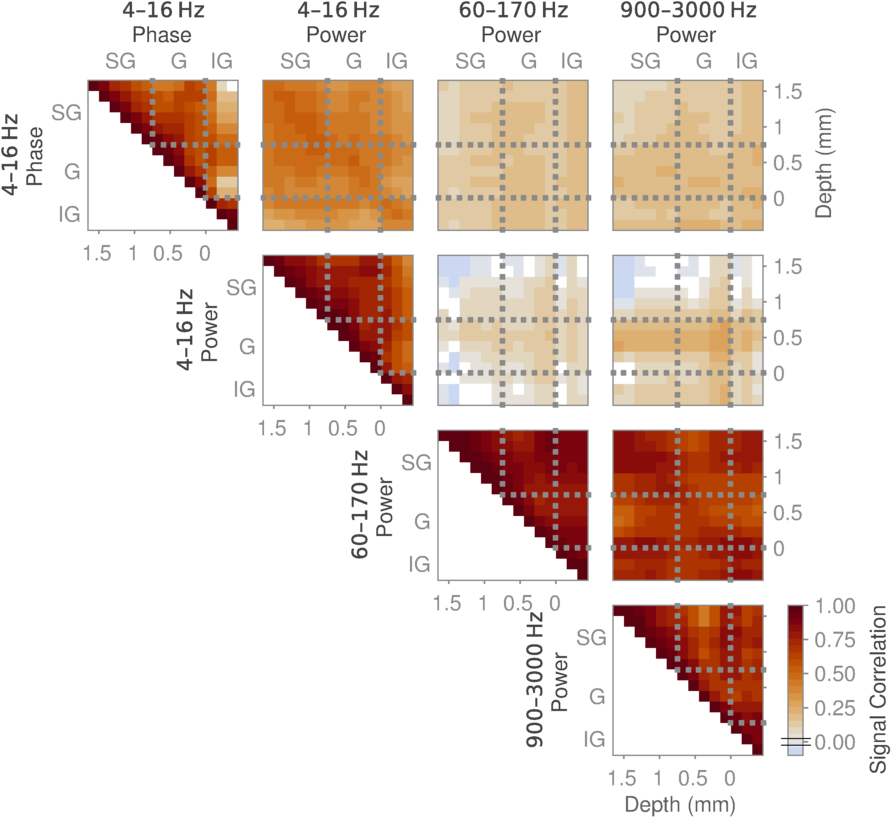
\includegraphics[scale=.5]{noisesigcorr/bndflt4-signal-avg_paper.png}
}
    \\
    \subfloat[Noise correlation\label{fig:lam_noise_corr_depth}]{
        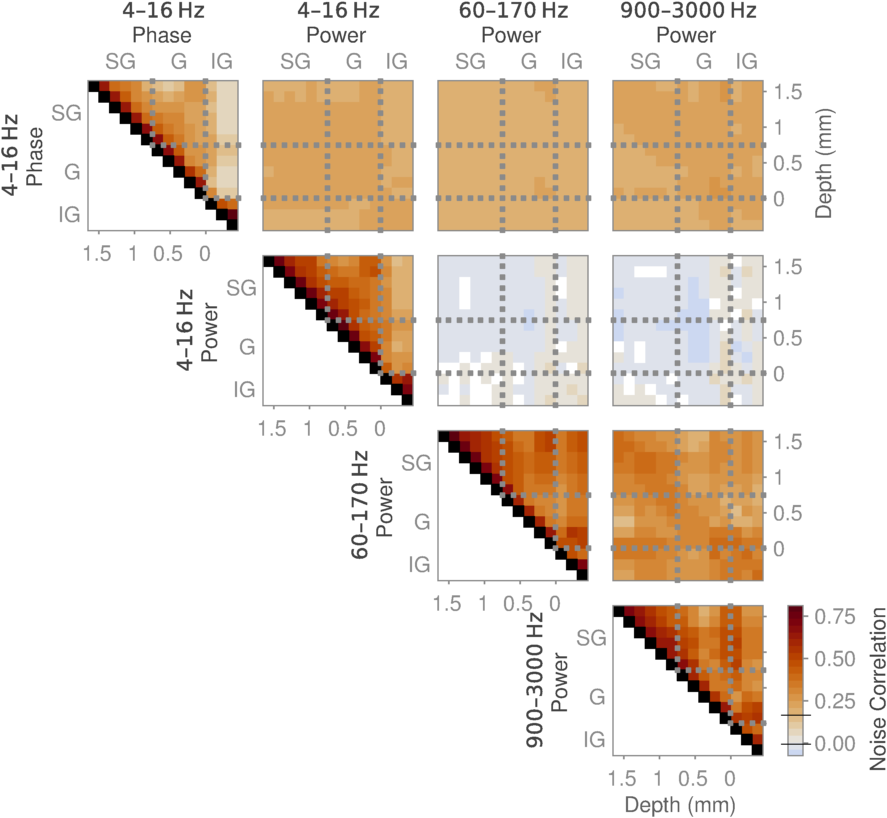
\includegraphics[scale=.5]{noisesigcorr/bndflt4-noise-avg_paper.png}
}
    \caption{
\protect\subref{fig:lam_signal_corr_depth}:~Signal correlation.
\protect\subref{fig:lam_noise_corr_depth}:~Noise correlation.
}
\label{fig:lam_noisesignal_corr_depth}
\end{figure}


\begin{figure}[htb]
    \centering
    \hspace*{\fill}
    \subfloat[Signal correlation\label{fig:lam_signal_corr_phase}]{
        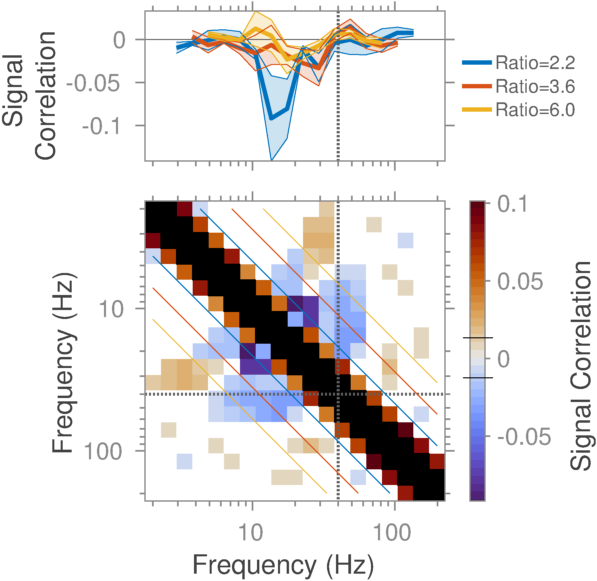
\includegraphics[scale=.45]{noisesigcorr/cxsfrq-signal-phase-phase-avg-log.png}
}
    \hspace*{\fill}\hspace{.2cm}\hspace*{\fill}
    \subfloat[Noise correlation\label{fig:lam_noise_corr_phase}]{
        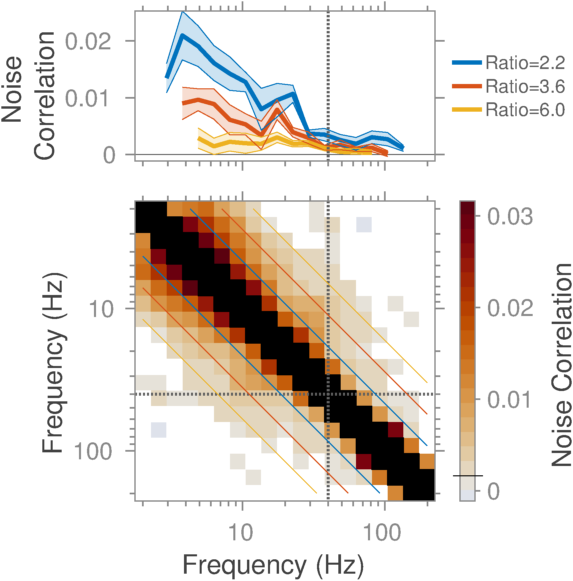
\includegraphics[scale=.45]{noisesigcorr/cxsfrq-noise-phase-phase-avg-log.png}
}
    \hspace*{\fill}
    \caption{Phase correlation
\protect\subref{fig:lam_signal_corr_phase}:~Signal correlation.
\protect\subref{fig:lam_noise_corr_phase}:~Noise correlation.
}
\label{fig:lam_noisesignal_corr_phase}
\end{figure}

\begin{figure}[htb]
    \centering
    \hspace*{\fill}
    \subfloat[Signal correlation\label{fig:lam_signal_corr_phase_power}]{
        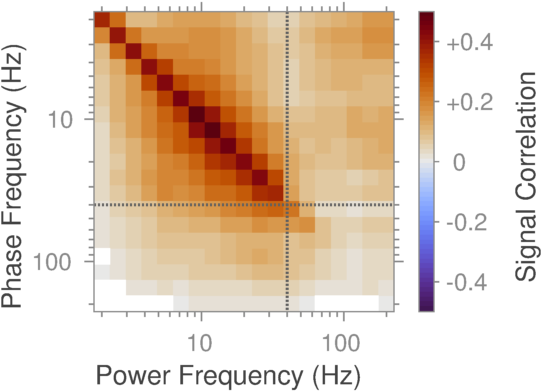
\includegraphics[scale=.45]{noisesigcorr/cxsfrq-signal-phase-power-avg-log.png}
}
    \hspace*{\fill}\hspace{.2cm}\hspace*{\fill}
    \subfloat[Noise correlation\label{fig:lam_noise_corr_phase_power}]{
        %\includegraphics[scale=.45]{noisesigcorr/cxsfrq-noise-phase-power-avg-log.png}
        <code running>
}
    \hspace*{\fill}
    \caption{Phase correlation with power
\protect\subref{fig:lam_signal_corr_phase_power}:~Signal correlation.
\protect\subref{fig:lam_noise_corr_phase_power}:~Noise correlation.
}
\label{fig:lam_noisesignal_corr_phase_power}
\end{figure}

Circular statistics were computed using the CircStat toolbox \citep{Berens2009}.

%-------------------------------------------------------------------------------
\FloatBarrier
\subsection{Phase correlation, \SIrange{4}{16}{Hz}}

Circular statistics were computed using the CircStat toolbox \citep{Berens2009}.

\begin{figure}[htb]
    \centering
    \hspace*{\fill}
    \subfloat[Movie driven\label{fig:lam_phasestats_alpha_line_csd_movie}]{
        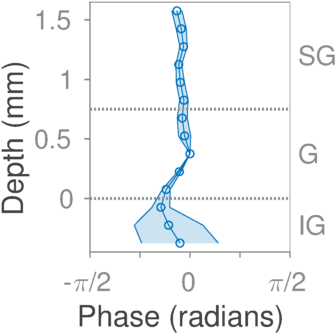
\includegraphics[scale=.45]{phasestats/movie1_Csd_phs4-16_dPhsTracebnd_5mean.png}
}
    \hspace*{\fill}\hspace{.2cm}\hspace*{\fill}
    \subfloat[Spontaneous\label{fig:lam_phasestats_alpha_line_csd_spont}]{
        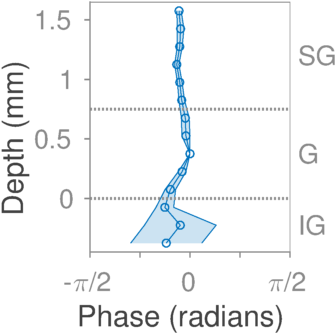
\includegraphics[scale=.45]{phasestats/spont_Csd_phs4-16_dPhsTracebnd_5mean.png}
}
    \hspace*{\fill}
    \caption{Phase correlation, \SIrange{4}{16}{Hz}.
\protect\subref{fig:lam_phasestats_alpha_line_csd_movie}:~Movie driven.
\protect\subref{fig:lam_phasestats_alpha_line_csd_spont}:~Spontaneous.
}
\label{fig:lam_phasestats_alpha_line_csd}
\end{figure}


\begin{figure}[htb]
    \centering
    \hspace*{\fill}
    \subfloat[Movie driven\label{fig:lam_phasestats_alpha_hist_csd_movie}]{
        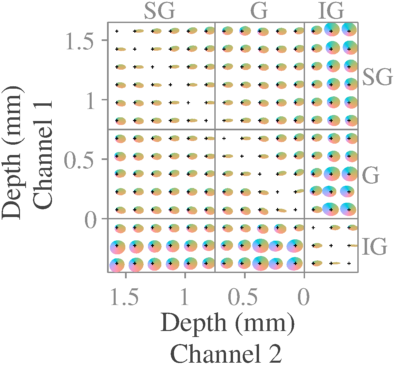
\includegraphics[scale=.45]{phasestats/movie1_Csd_phs4-16_dPhs_hist_5mean.png}
}
    \hspace*{\fill}\hspace{.2cm}\hspace*{\fill}
    \subfloat[Spontaneous\label{fig:lam_phasestats_alpha_hist_csd_spont}]{
        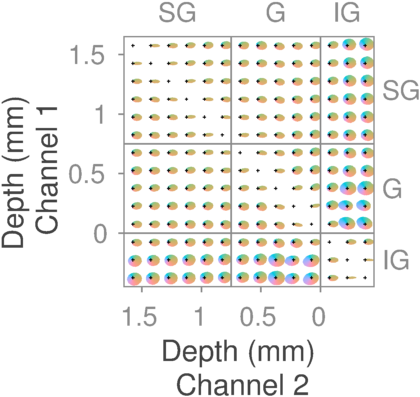
\includegraphics[scale=.45]{phasestats/spont_Csd_phs4-16_dPhs_hist_5mean.png}
}
    \hspace*{\fill}
    \caption{Phase correlation, \SIrange{4}{16}{Hz}.
\protect\subref{fig:lam_phasestats_alpha_hist_csd_movie}:~Movie driven.
\protect\subref{fig:lam_phasestats_alpha_hist_csd_spont}:~Spontaneous.
}
\label{fig:lam_phasestats_alpha_hist_csd}
\end{figure}


\begin{figure}[htb]
    \centering
    \hspace*{\fill}
    \subfloat[Movie driven\label{fig:lam_phasestats_alpha_combo_csd_movie}]{
        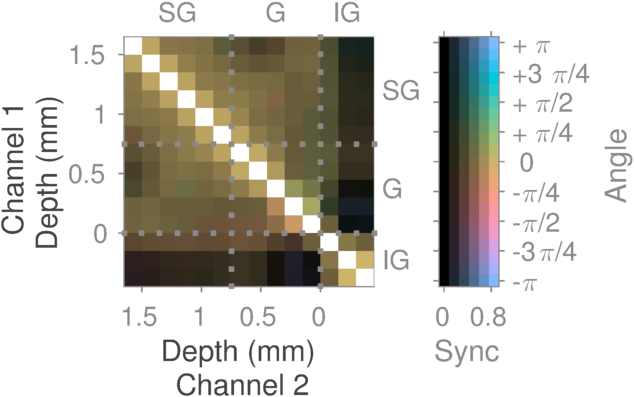
\includegraphics[scale=.45]{phasestats/movie1_Csd_phs4-16_dPhs_combo_5mean.png}
}
    \hspace*{\fill}\hspace{.2cm}\hspace*{\fill}
    \subfloat[Spontaneous\label{fig:lam_phasestats_alpha_combo_csd_spont}]{
        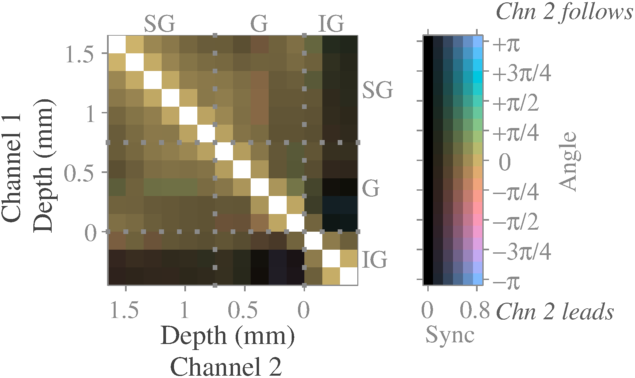
\includegraphics[scale=.45]{phasestats/spont_Csd_phs4-16_dPhs_combo_5mean.png}
}
    \hspace*{\fill}
    \caption{Phase correlation, showing phase offset and synchronicity \SIrange{4}{16}{Hz}.
\protect\subref{fig:lam_phasestats_alpha_combo_csd_movie}:~Movie driven.
\protect\subref{fig:lam_phasestats_alpha_combo_csd_spont}:~Spontaneous.
}
\label{fig:lam_phasestats_alpha_combo_csd}
\end{figure}


\begin{figure}[htb]
    \centering
    \hspace*{\fill}
    \subfloat[Movie driven\label{fig:lam_phasestats_alpha_summary_csd_movie}]{
        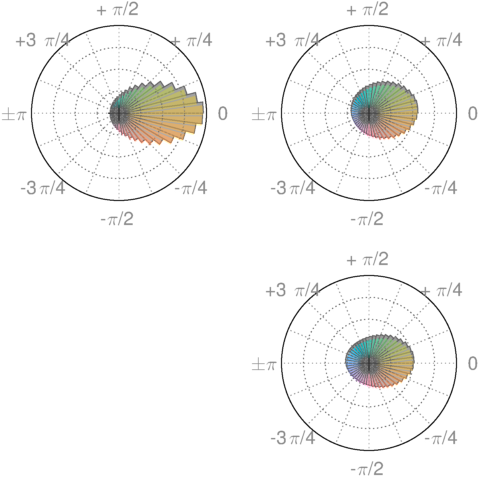
\includegraphics[scale=.45]{phasestats/movie1_Csd_simplephs4-16_dPhs_hist.png}
}
    \hspace*{\fill}\hspace{.2cm}\hspace*{\fill}
    \subfloat[Spontaneous\label{fig:lam_phasestats_alpha_summary_csd_spont}]{
        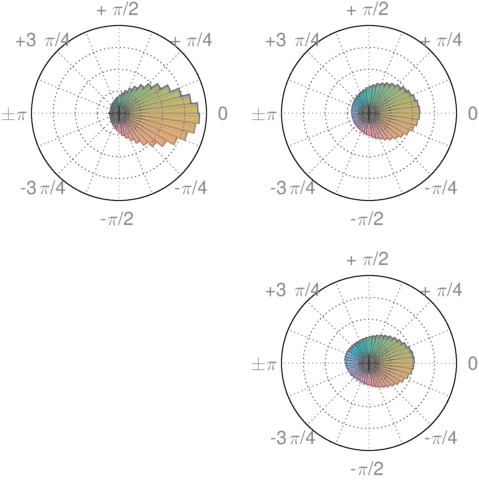
\includegraphics[scale=.45]{phasestats/spont_Csd_simplephs4-16_dPhs_hist.png}
}
    \hspace*{\fill}
    \caption{Phase correlation, summary by region, \SIrange{4}{16}{Hz}.
\protect\subref{fig:lam_phasestats_alpha_summary_csd_movie}:~Movie driven.
\protect\subref{fig:lam_phasestats_alpha_summary_csd_spont}:~Spontaneous.
}
\label{fig:lam_phasestats_alpha_summary_csd}
\end{figure}

%-------------------------------------------------------------------------------
\FloatBarrier
\subsection{Phase correlation, \SIrange{60}{170}{Hz}}

Circular statistics were computed using the CircStat toolbox \citep{Berens2009}.

\begin{figure}[htb]
    \centering
    \hspace*{\fill}
    \subfloat[Movie driven\label{fig:lam_phasestats_gamma_line_csd_movie}]{
        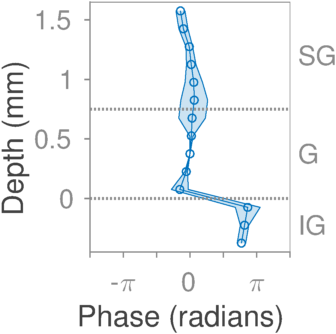
\includegraphics[scale=.45]{phasestats/movie1_Csd_phs60-170_dPhsTracebnd_5mean.png}
}
    \hspace*{\fill}\hspace{.2cm}\hspace*{\fill}
    \subfloat[Spontaneous\label{fig:lam_phasestats_gamma_line_csd_spont}]{
        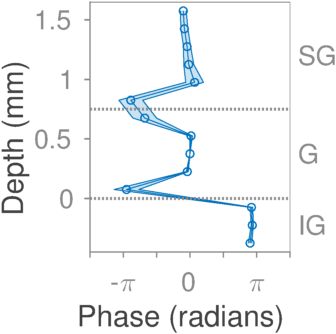
\includegraphics[scale=.45]{phasestats/spont_Csd_phs60-170_dPhsTracebnd_5mean.png}
}
    \hspace*{\fill}
    \caption{Phase correlation, \SIrange{60}{170}{Hz}.
\protect\subref{fig:lam_phasestats_gamma_line_csd_movie}:~Movie driven.
\protect\subref{fig:lam_phasestats_gamma_line_csd_spont}:~Spontaneous.
}
\label{fig:lam_phasestats_gamma_line_csd}
\end{figure}


\begin{figure}[htb]
    \centering
    \hspace*{\fill}
    \subfloat[Movie driven\label{fig:lam_phasestats_gamma_hist_csd_movie}]{
        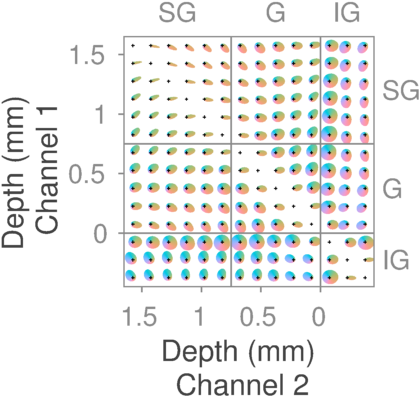
\includegraphics[scale=.45]{phasestats/movie1_Csd_phs60-170_dPhs_hist_5mean.png}
}
    \hspace*{\fill}\hspace{.2cm}\hspace*{\fill}
    \subfloat[Spontaneous\label{fig:lam_phasestats_gamma_hist_csd_spont}]{
        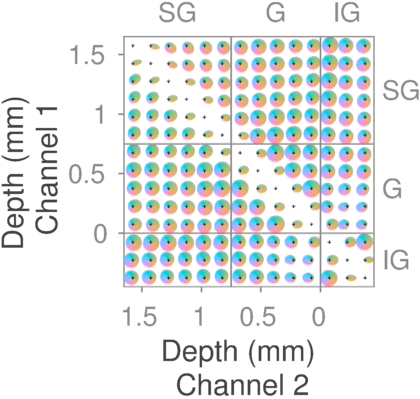
\includegraphics[scale=.45]{phasestats/spont_Csd_phs60-170_dPhs_hist_5mean.png}
}
    \hspace*{\fill}
    \caption{Phase correlation, \SIrange{60}{170}{Hz}.
\protect\subref{fig:lam_phasestats_gamma_hist_csd_movie}:~Movie driven.
\protect\subref{fig:lam_phasestats_gamma_hist_csd_spont}:~Spontaneous.
}
\label{fig:lam_phasestats_gamma_hist_csd}
\end{figure}


\begin{figure}[htb]
    \centering
    \hspace*{\fill}
    \subfloat[Movie driven\label{fig:lam_phasestats_gamma_combo_csd_movie}]{
        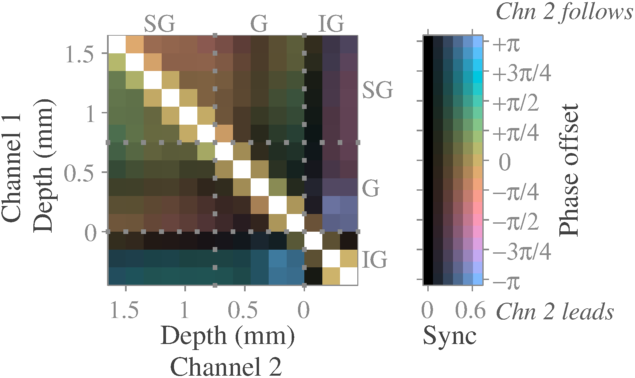
\includegraphics[scale=.45]{phasestats/movie1_Csd_phs60-170_dPhs_combo_5mean.png}
}
    \hspace*{\fill}\hspace{.2cm}\hspace*{\fill}
    \subfloat[Spontaneous\label{fig:lam_phasestats_gamma_combo_csd_spont}]{
        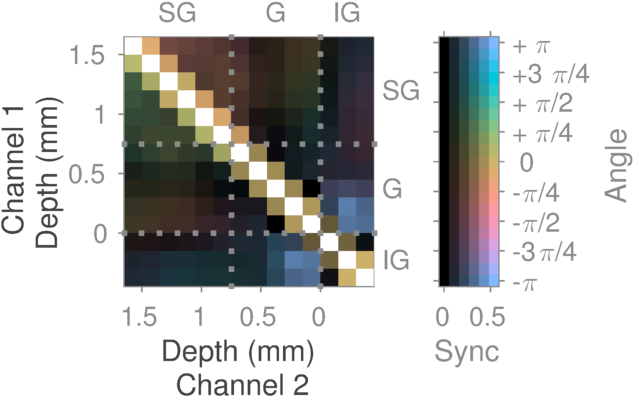
\includegraphics[scale=.45]{phasestats/spont_Csd_phs60-170_dPhs_combo_5mean.png}
}
    \hspace*{\fill}
    \caption{Phase correlation, showing phase offset and synchronicity \SIrange{60}{170}{Hz}.
\protect\subref{fig:lam_phasestats_gamma_combo_csd_movie}:~Movie driven.
\protect\subref{fig:lam_phasestats_gamma_combo_csd_spont}:~Spontaneous.
}
\label{fig:lam_phasestats_gamma_combo_csd}
\end{figure}


\begin{figure}[htb]
    \centering
    \hspace*{\fill}
    \subfloat[Movie driven\label{fig:lam_phasestats_gamma_summary_csd_movie}]{
        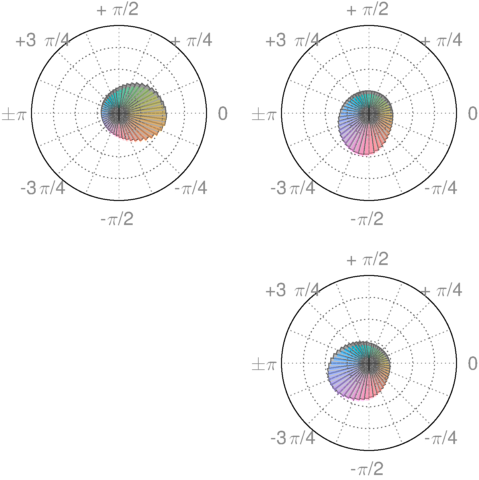
\includegraphics[scale=.45]{phasestats/movie1_Csd_simplephs60-170_dPhs_hist.png}
}
    \hspace*{\fill}\hspace{.2cm}\hspace*{\fill}
    \subfloat[Spontaneous\label{fig:lam_phasestats_gamma_summary_csd_spont}]{
        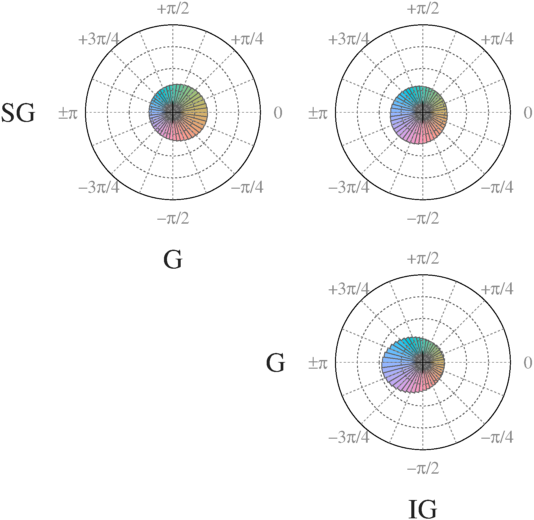
\includegraphics[scale=.45]{phasestats/spont_Csd_simplephs60-170_dPhs_hist.png}
}
    \hspace*{\fill}
    \caption{Phase correlation, summary by region, \SIrange{60}{170}{Hz}.
\protect\subref{fig:lam_phasestats_gamma_summary_csd_movie}:~Movie driven.
\protect\subref{fig:lam_phasestats_gamma_summary_csd_spont}:~Spontaneous.
}
\label{fig:lam_phasestats_gamma_summary_csd}
\end{figure}


%-------------------------------------------------------------------------------
\FloatBarrier
\subsection{Stimulus information contained in phase}

\begin{figure}[htb]
    \centering
    \subfloat[\ac{LFP}\label{fig:lam_phase_info_lfp}]{
        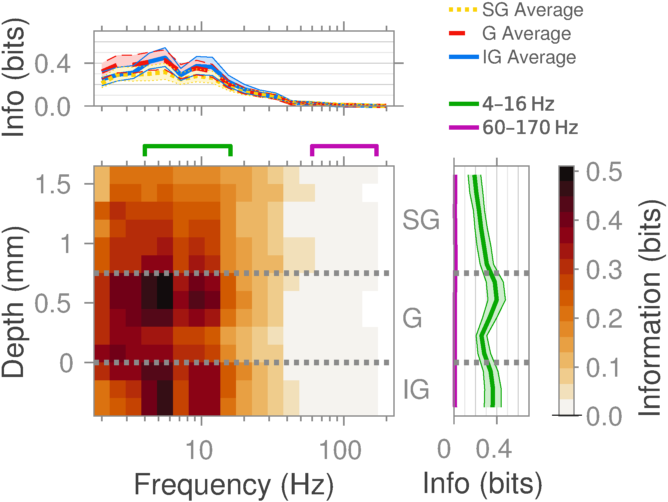
\includegraphics[scale=.5]{phaseinfo/fig3set-info-Csd-phase-straightnanmean-compzonescb-legend.png}
}
    \\
    \subfloat[\ac{CSD}\label{fig:lam_phase_info_csd}]{
        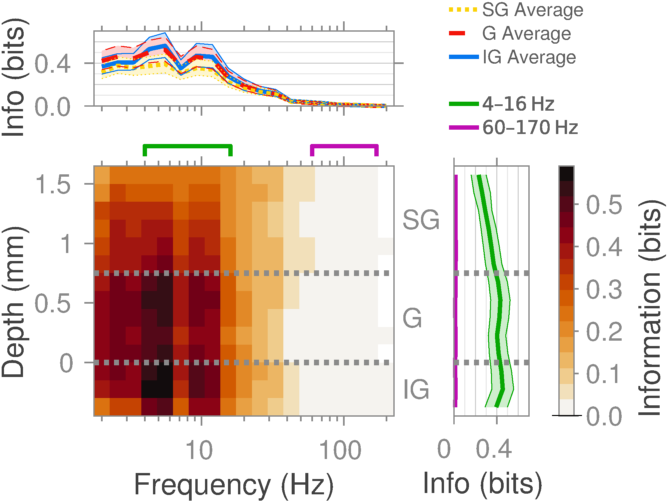
\includegraphics[scale=.5]{phaseinfo/fig3set-info-Cln-phase-straightnanmean-compzonescb-legend.png}
}
    \caption{
Information about the stimulus contained in the phase of the extracellular neural signal, as a function of frequency. Mean of 6 sessions.
\protect\subref{fig:lam_phase_info_lfp}:~\ac{LFP}.
\protect\subref{fig:lam_phase_info_csd}:~\ac{CSD}.
}
\label{fig:lam_phase_info}
\end{figure}


\begin{figure}[htb]
    \centering
    \hspace*{\fill}
    \subfloat[\sesname{H05391}\label{fig:lam_phase_info_lfp_H05391}]{
        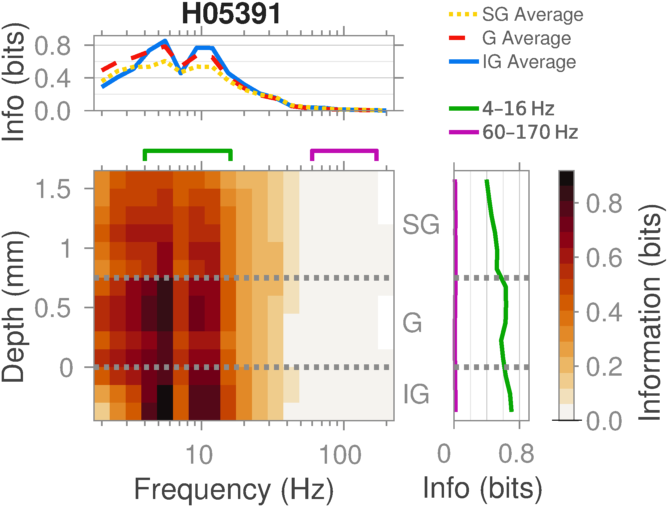
\includegraphics[scale=.4]{phaseinfo/fig3set-info-Cln-phase-H05391-compzonescb-legend.png}
}
    \hspace*{\fill}\hspace{.2cm}\hspace*{\fill}
    \subfloat[\sesname{H05nm9}\label{fig:lam_phase_info_lfp_H05nm9}]{
        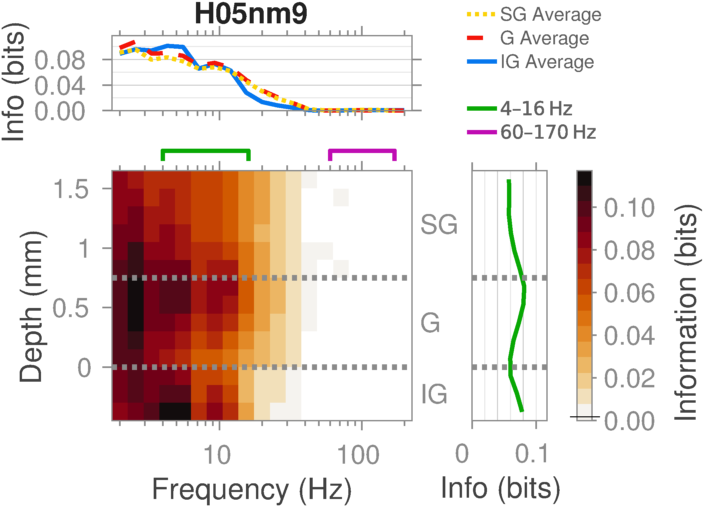
\includegraphics[scale=.4]{phaseinfo/fig3set-info-Cln-phase-H05nm9-compzonescb-legend.png}
}
    \hspace*{\fill}
    \\
    \hspace*{\fill}
    \subfloat[\sesname{H05nm7}\label{fig:lam_phase_info_lfp_H05nm7}]{
        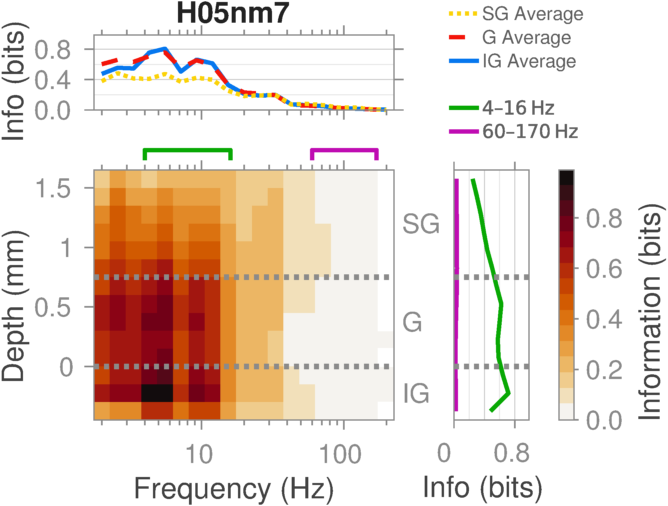
\includegraphics[scale=.4]{phaseinfo/fig3set-info-Cln-phase-H05nm7-compzonescb-legend.png}
}
    \hspace*{\fill}\hspace{.2cm}\hspace*{\fill}
    \subfloat[\sesname{E07nm1}\label{fig:lam_phase_info_lfp_E07nm1}]{
        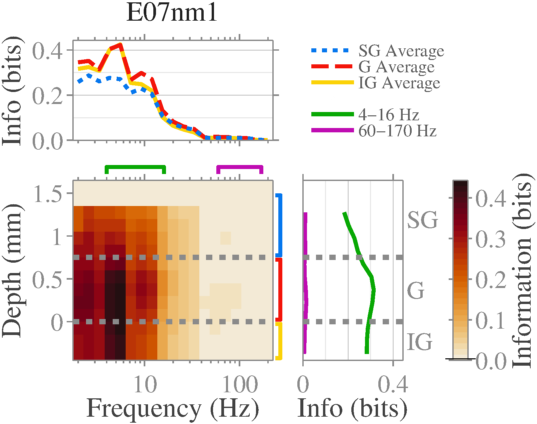
\includegraphics[scale=.4]{phaseinfo/fig3set-info-Cln-phase-E07nm1-compzonescb-legend.png}
}
    \hspace*{\fill}
    \\
    \hspace*{\fill}
    \subfloat[\sesname{F10nm1}\label{fig:lam_phase_info_lfp_F10nm1}]{
        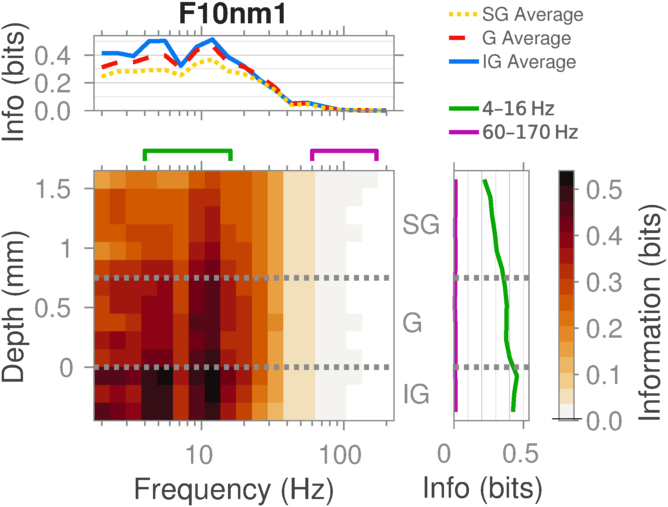
\includegraphics[scale=.4]{phaseinfo/fig3set-info-Cln-phase-F10nm1-compzonescb-legend.png}
}
    \hspace*{\fill}\hspace{.2cm}\hspace*{\fill}
    \subfloat[\sesname{J10nm1}\label{fig:lam_phase_info_lfp_J10nm1}]{
        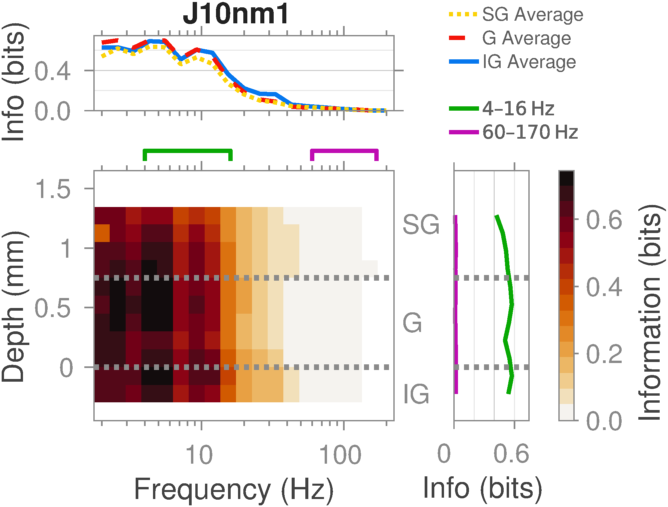
\includegraphics[scale=.4]{phaseinfo/fig3set-info-Cln-phase-J10nm1-compzonescb-legend.png}
}
    \hspace*{\fill}
    \caption{
Information about the stimulus contained in the phase of the \ac{LFP}, as a function of frequency, by session.
}
\label{fig:lam_phase_info_lfp_sessions}
\end{figure}


\begin{figure}[htb]
    \centering
    \hspace*{\fill}
    \subfloat[\sesname{H05391}\label{fig:lam_phase_info_csd_H05391}]{
        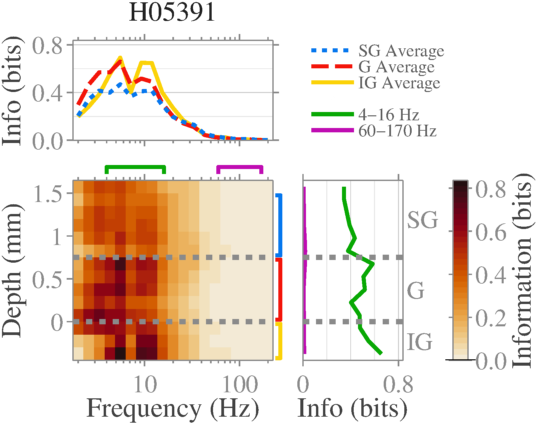
\includegraphics[scale=.4]{phaseinfo/fig3set-info-Csd-phase-H05391-compzonescb-legend.png}
}
    \hspace*{\fill}\hspace{.2cm}\hspace*{\fill}
    \subfloat[\sesname{H05nm9}\label{fig:lam_phase_info_csd_H05nm9}]{
        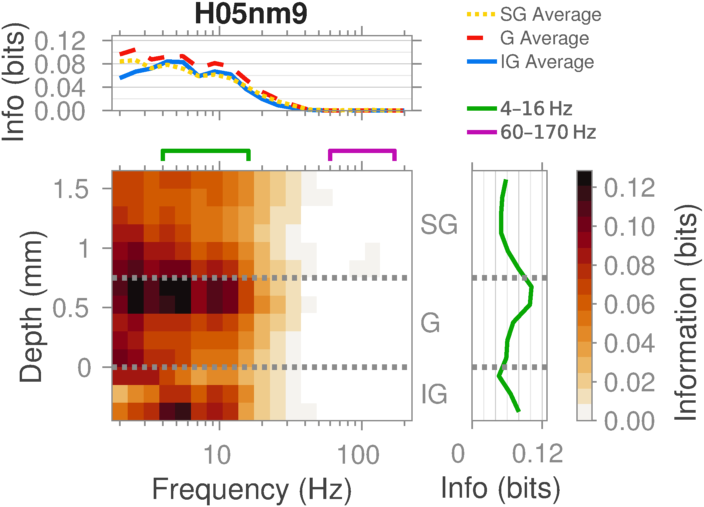
\includegraphics[scale=.4]{phaseinfo/fig3set-info-Csd-phase-H05nm9-compzonescb-legend.png}
}
    \hspace*{\fill}
    \\
    \hspace*{\fill}
    \subfloat[\sesname{H05nm7}\label{fig:lam_phase_info_csd_H05nm7}]{
        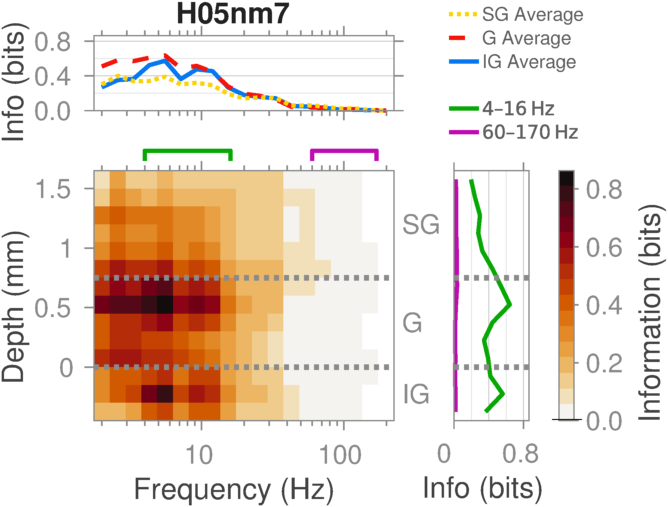
\includegraphics[scale=.4]{phaseinfo/fig3set-info-Csd-phase-H05nm7-compzonescb-legend.png}
}
    \hspace*{\fill}\hspace{.2cm}\hspace*{\fill}
    \subfloat[\sesname{E07nm1}\label{fig:lam_phase_info_csd_E07nm1}]{
        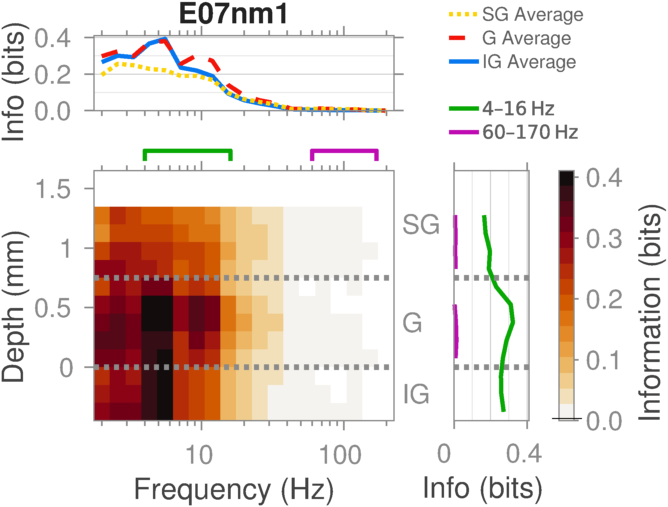
\includegraphics[scale=.4]{phaseinfo/fig3set-info-Csd-phase-E07nm1-compzonescb-legend.png}
}
    \hspace*{\fill}
    \\
    \hspace*{\fill}
    \subfloat[\sesname{F10nm1}\label{fig:lam_phase_info_csd_F10nm1}]{
        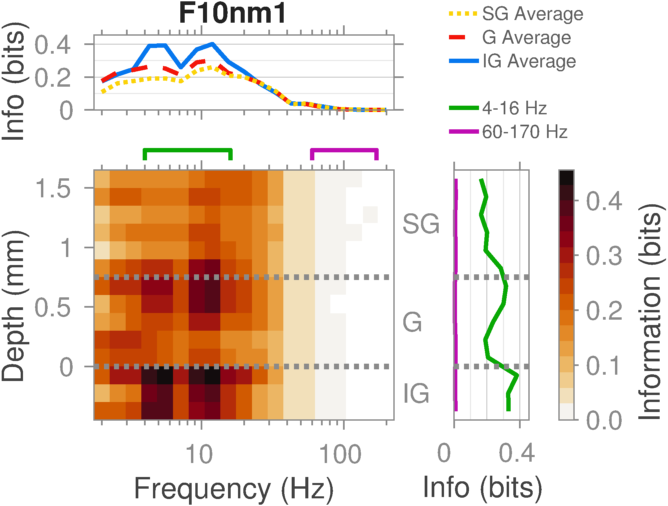
\includegraphics[scale=.4]{phaseinfo/fig3set-info-Csd-phase-F10nm1-compzonescb-legend.png}
}
    \hspace*{\fill}\hspace{.2cm}\hspace*{\fill}
    \subfloat[\sesname{J10nm1}\label{fig:lam_phase_info_csd_J10nm1}]{
        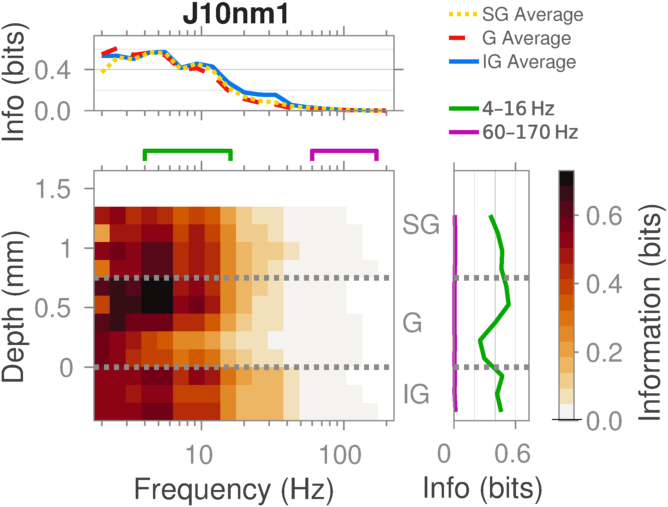
\includegraphics[scale=.4]{phaseinfo/fig3set-info-Csd-phase-J10nm1-compzonescb-legend.png}
}
    \hspace*{\fill}
    \caption{
Information about the stimulus contained in the phase of the \ac{CSD}, as a function of frequency, by session.
}
\label{fig:lam_phase_info_csd_sessions}
\end{figure}


%-------------------------------------------------------------------------------
\FloatBarrier
\subsection{Redundancy}

%-------------------------------------------------------------------------------


We define redundancy as
\begin{equation}
\label{eq:red}
\operatorname{Redundancy}\left(X,Y;S\right)=\frac{
\I\left(X;S\right) + \I\left(Y;S\right) - \I\left(\left\{X,Y\right\};S\right)
}{
\I\left(\left\{X,Y\right\};S\right)
},
\end{equation}
where $S$ is the stimulus, and $X$ and $Y$ are observed responses.
If $\operatorname{Redundancy}\left(X,Y;S\right) > 0$, this implies that $X$ and $Y$ contain redundant information about $S$.
If $\operatorname{Redundancy}\left(X,Y;S\right) < 0$, then $X$ and $Y$ are synergistic, such that knowing the paired state of $X$ and $Y$ simultaneously contains more information about $S$ than one would expect from the information just contained in $X$ and $Y$ individually.

Unfortunately, since redundant and synergistic information co-occur when transitioning from knowing either $X$ or $Y$ to knowing the state $(X,Y)$, it is not possible to quantify the redundancy and synergy in isolation.
The term which we refer to as ``Redundancy'' in \autoref{eq:red}, is in reality the difference of the true (but unobservable) redundancy and synergy about $S$ in $X$ and $Y$.
Consequently, we can only conclude how much more redundancy than synergy there is, and when redundancy exceeds synergy that there is at least some redundancy.
For instance, in the case $\operatorname{Redundancy}\left(X,Y;S\right) = 0$, we can only conclude that there is the same amount of synergy as redundancy; it is not necessarily the case that $X$ and $Y$ contain exclusively independent information about $S$.


We define (relative) information gain as
% \begin{equation}
% \operatorname{InfoGain}\left(X,Y;S\right)=\frac{
% \I\left(\left\{i1,i2\right\};S\right) - \I\left(i1;S\right)
% }{
% \I\left(i2;S\right)
% }
% \end{equation}
\begin{equation}
\operatorname{InfoGain}\left(Y\to\left\{X,Y\right\};S\right)=\frac{
\I\left(\left\{X,Y\right\};S\right) - \I\left(Y;S\right)
}{
\I\left(X;S\right)
},
\end{equation}
which is the amount of information gained about the stimulus when we already know $Y$ and $X$ is revealed to us, relative to the amount of information about the stimulus contained in $X$.
If $X$ contains no more information about $S$ than is already contained in $Y$, then
$\I\left(\left\{X,Y\right\};S\right) = \I\left(Y;S\right)$
and we therefore have
$$\operatorname{InfoGain}\left(Y\to\left\{X,Y\right\};S\right)=0 ,$$
which makes intuitive sense in line with the concept of information gain.
However, if $\I\left(X;S\right)=0$, meaning $X$ contains no information about the stimulus, this would be divergent, so we instead choose by definition
$$\operatorname{InfoGain}\left(Y\to\left\{X,Y\right\};S\right)=0$$
for this case.
If $X$ and $Y$ contain independent information about the stimulus,
$\I\left(\left\{X,Y\right\};S\right) = \I\left(X;S\right) + \I\left(Y;S\right)$,
then we find that
$$\operatorname{InfoGain}\left(Y\to\left\{X,Y\right\};S\right) = 1 = 100\%.$$
However, as stated above, observing
$\operatorname{InfoGain} = 1$
is necessary but insufficient to conclude that $X$ and $Y$ contain exclusively independent information about $S$, since the same result can be achieved provided their synergy and redundancy effects cancel each other out.
Should $X$ and $Y$ contain more synergistic than redundant information about $S$, we will observe a relative information gain exceeding $1$ (or equivalently $100\%$).


\subsubsection{Cross channel}

\begin{figure}[htb]
    \centering
    \subfloat[\label{fig:lam_phase_cxchn_info_red}]{
        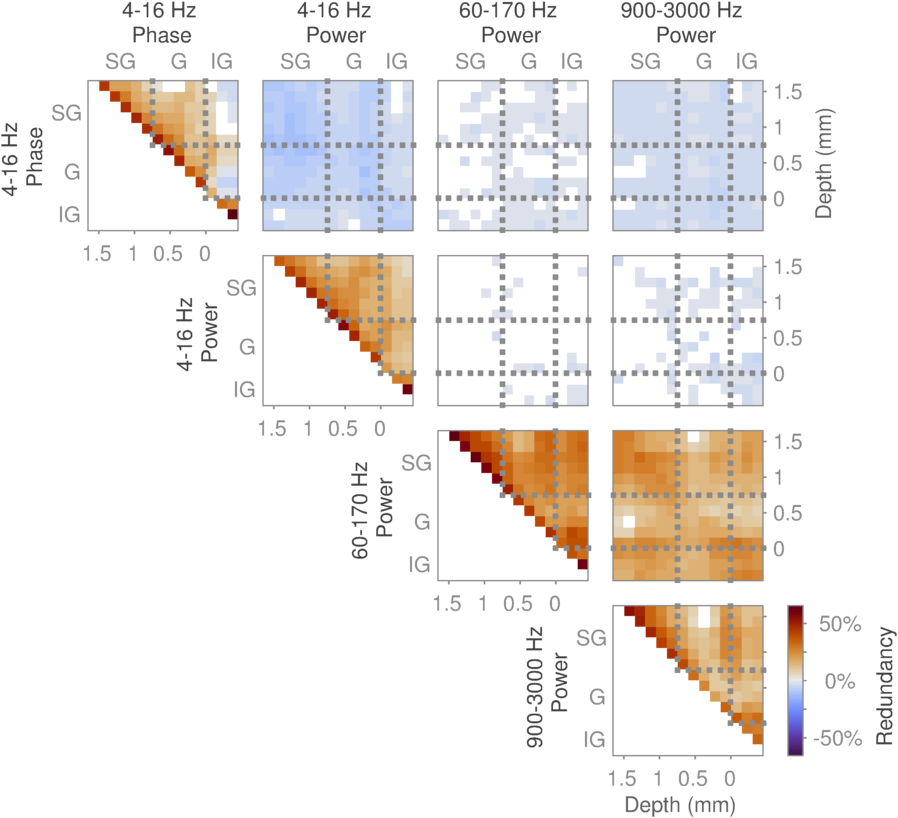
\includegraphics[scale=.5]{redundancy-cxschn/bndflt4-PCred-none-avg-lag=0s_paper.png}
}
    \\
    \subfloat[\label{fig:lam_phase_cxchn_info_red_bar}]{
        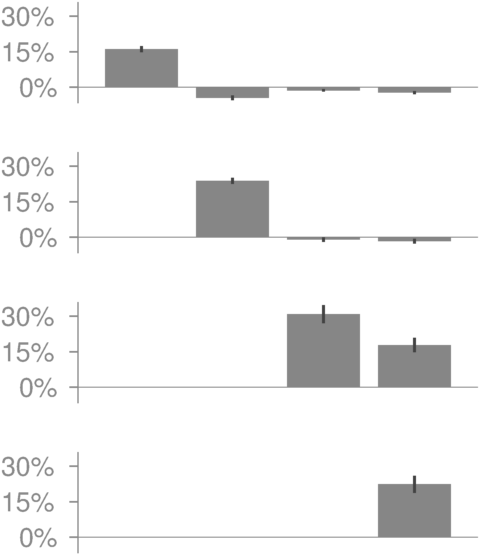
\includegraphics[scale=.5]{redundancy-cxschn/bndflt-barplot4_PCred-none-avg_lag=0s_paper.png}
}
    \caption{Redundancy of bands across channels.
}
\label{fig:lam_phase_cxchn_info_red_overall}
\end{figure}


\begin{figure}[htb]
    \centering
    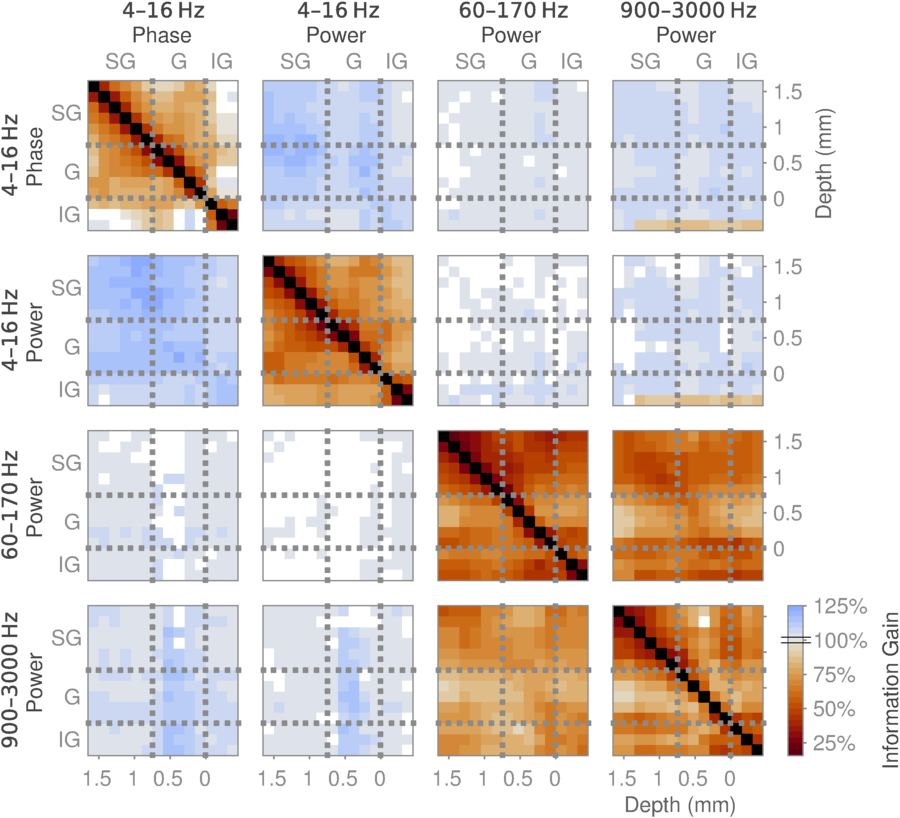
\includegraphics[scale=.5]{redundancy-cxschn/bndflt4-PCgain-i2d2-none-avg-lag=0s_paper.png}
    \caption{Information gain between bands across channels.
}
\label{fig:lam_phase_cxchn_info_gain}
\end{figure}

%-------------------------------------------------------------------------------
\subsubsection{Cross frequency}

\begin{figure}[htb]
    \centering
    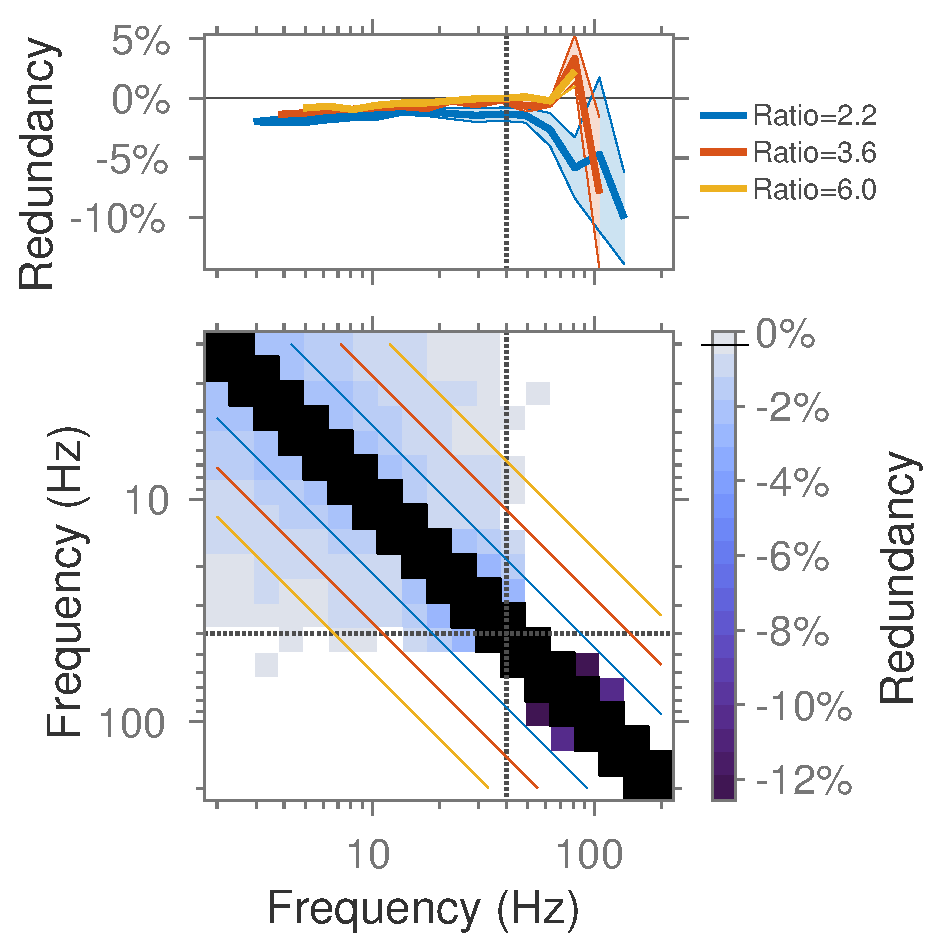
\includegraphics[scale=.5]{redundancy-cxsfrq/cxsfrq-PCred_phase-phase_avg-log}
    \caption{
Redundancy between frequencies.
}
\label{fig:lam_phase_cxfrq_info_red}
\end{figure}

\begin{figure}[htb]
    \centering
    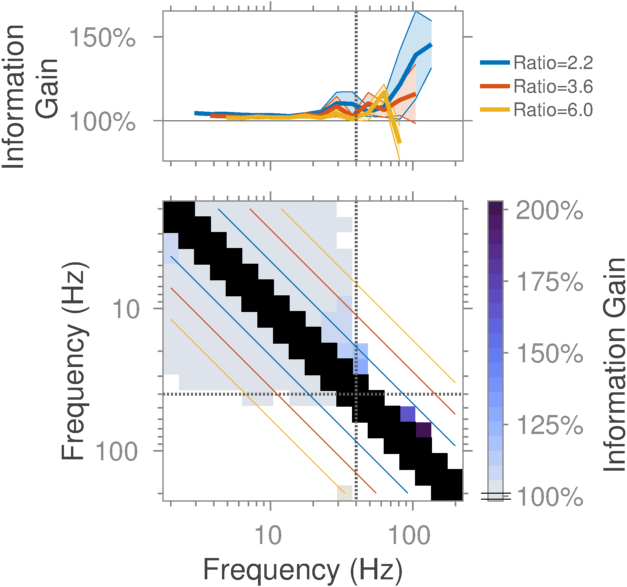
\includegraphics[scale=.5]{redundancy-cxsfrq/cxsfrq-PCgain-i2d2_phase-phase_avg-log}
    \caption{
Information gain between frequencies.
}
\label{fig:lam_phase_cxfrq_info_gain}
\end{figure}

%-------------------------------------------------------------------------------
\subsubsection{Cross frequency phase vs power}

\begin{figure}[htb]
    \centering
    \subfloat[\label{fig:lam_cxfrq_powerphase_info_red_hm}]{
        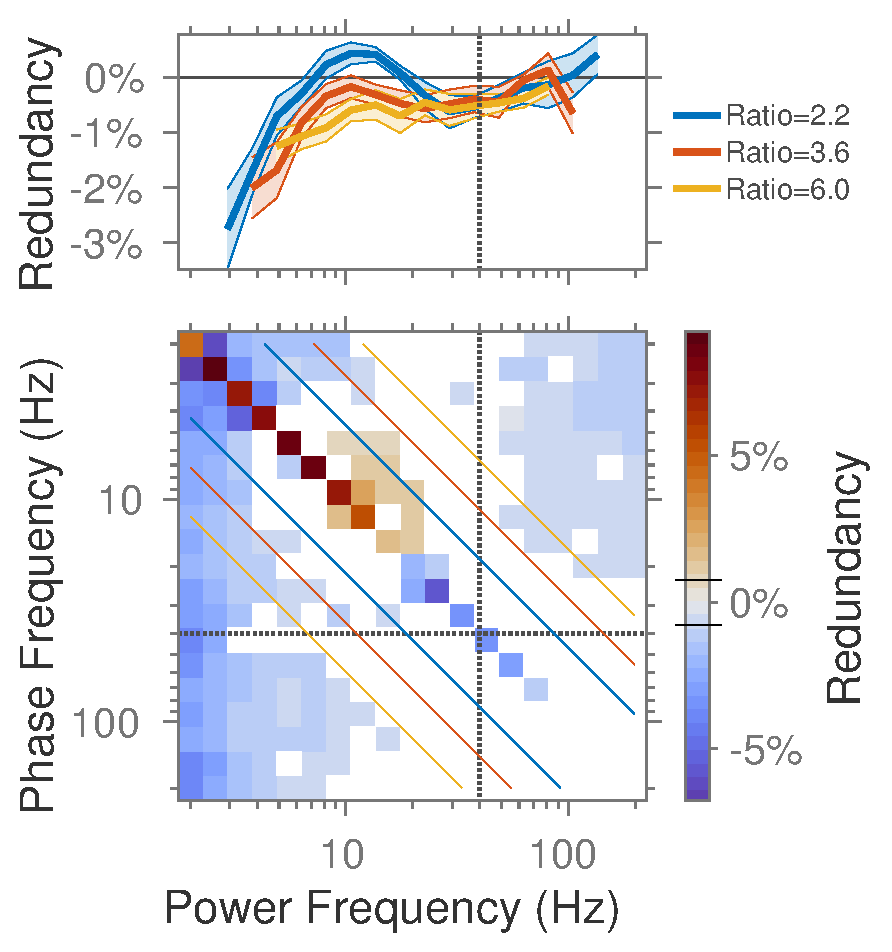
\includegraphics[scale=.5]{redundancy-cxsfrq/cxsfrq-PCred_phase-power_avg-log}
}
    \\
    \subfloat[\label{fig:lam_cxfrq_powerphase_info_red_bar}]{
        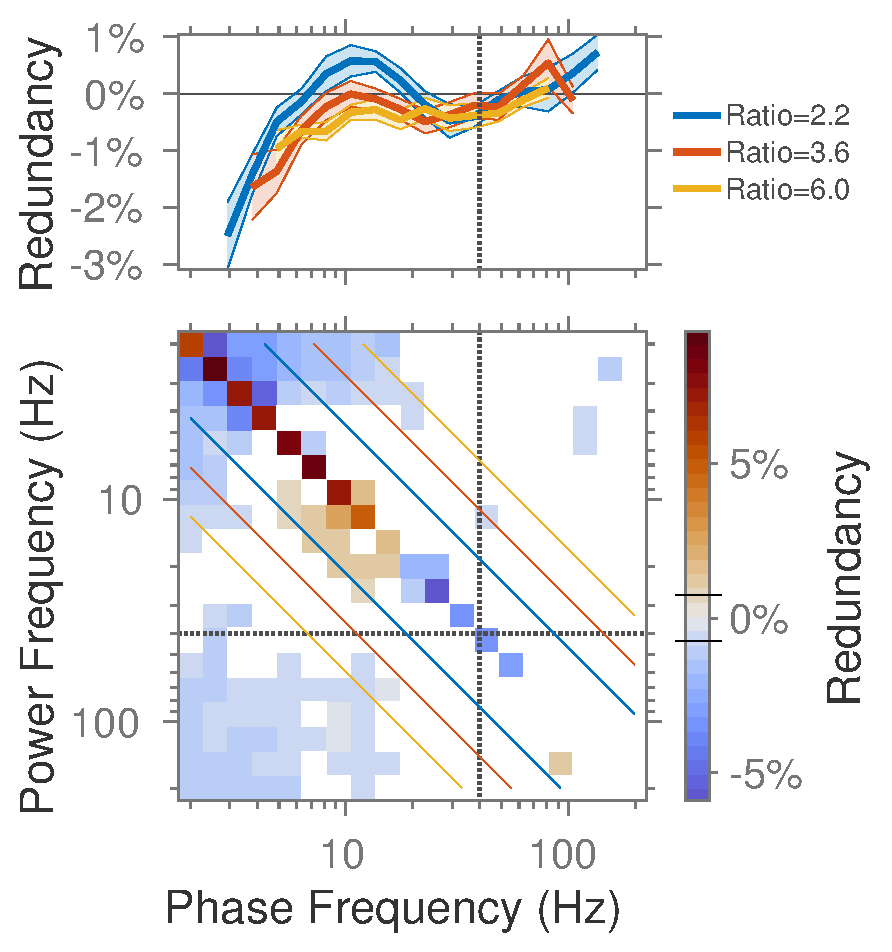
\includegraphics[scale=.5]{redundancy-cxsfrq/cxsfrq-PCred_power-phase_avg-log}
}
    \caption{
Redundancy between frequencies.
}
\label{fig:lam_cxfrq_powerphase_info_red}
\end{figure}



\begin{figure}[htb]
    \centering
    \subfloat[\label{fig:lam_cxfrq_powerphase_info_gain_hm}]{
        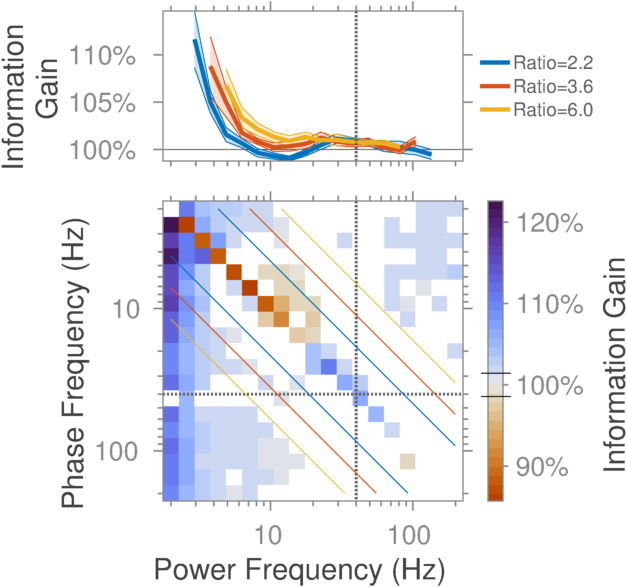
\includegraphics[scale=.5]{redundancy-cxsfrq/cxsfrq-PCgain-i2d2_phase-power_avg-log}
}
    \\
    \subfloat[\label{fig:lam_cxfrq_powerphase_info_gain_bar}]{
        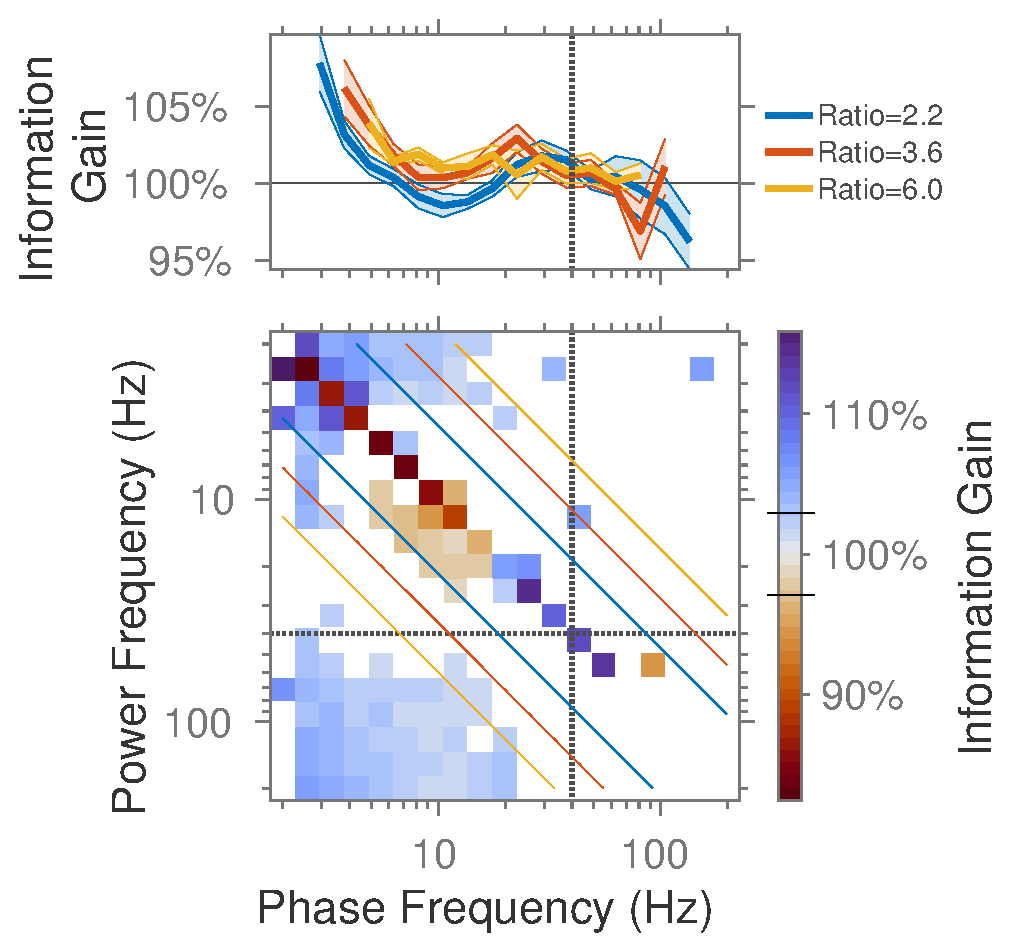
\includegraphics[scale=.5]{redundancy-cxsfrq/cxsfrq-PCgain-i2d2_power-phase_avg-log}
}
    \caption{
Information gain between frequencies.
}
\label{fig:lam_cxfrq_powerphase_info_gain}
\end{figure}

%-------------------------------------------------------------------------------
\section{Discussion}
%-------------------------------------------------------------------------------
